% Standard Article Definition
\documentclass[]{article}

% Page Formatting
\usepackage[margin=1in]{geometry}
\setlength\parindent{0pt}

% Graphics
\usepackage{graphicx}

% Math Packages
\usepackage{physics}
\usepackage{amsmath, amsfonts, amssymb, amsthm}
\usepackage{mathtools}

% Extra Packages
\usepackage{pdfpages}
\usepackage{hyperref}
% \usepackage{listings}

% Section Heading Settings
% \usepackage{enumitem}
% \renewcommand{\theenumi}{\alph{enumi}}
\renewcommand*{\thesection}{Problem \arabic{section}}
\renewcommand*{\thesubsection}{\arabic{section}\alph{subsection})}
\renewcommand*{\thesubsubsection}{}%\quad \quad \roman{subsubsection})}

\newcommand{\Problem}{\subsubsection*{\textbf{PROBLEM:}}}
\newcommand{\Solution}{\subsubsection*{\textbf{SOLUTION:}}}
\newcommand{\Preliminaries}{\subsubsection*{\textbf{PRELIMINARIES:}}}

%Custom Commands
\newcommand{\N}{\mathbb{N}}
\newcommand{\Z}{\mathbb{Z}}
% \newcommand{\Q}{\mathbb{Q}}
\newcommand{\R}{\mathbb{R}}
\newcommand{\C}{\mathbb{C}}

% \newcommand{\SigAlg}{\mathcal{S}}

% \newcommand{\Rel}{\mathcal{R}}

% \newcommand{\toI}{\xrightarrow{\textsf{\tiny I}}}
% \newcommand{\toS}{\xrightarrow{\textsf{\tiny S}}}
% \newcommand{\toB}{\xrightarrow{\textsf{\tiny B}}}

% \newcommand{\divisible}{ \ \vdots \ }
\newcommand{\st}{\ : \ }

% Theorem Definition
\newtheorem{definition}{Definition}
\newtheorem{assumption}{Assumption}
\newtheorem{theorem}{Theorem}
\newtheorem{lemma}{Lemma}
\newtheorem{proposition}{Proposition}
\newtheorem{remark}{Remark}
% \newtheorem{example}{Example}
% \newtheorem{counterExample}{Counter Example}


%opening
\title{
    MECH 6326 - Optimal Control and Dynamic Programming \\ 
    Homework 4
}
\author{Jonas Wagner\\ jonas.wagner@utdallas.edu}
\date{2023, April 13\textsuperscript{th}}

\begin{document}

\maketitle

\tableofcontents

\newpage
\textbf{Dynamic Programming Implementation for Markov Decision Process}
% Problem 1 ----------------------------------------------
\section{Robot navigation in an uncertain environment} 
\Problem
You are designing a controller to navigate a robot through a cluttered and uncertain environment. 
We use a very simplified 2D grid model, where the robot starts in the bottom-left corner, and must move to the top-right corner, and can move either up or to the right at each step.
Due to unpredictable robot-environment interaction, if the robot moves in the same direction as in the previous time-step, there is a higher probability of moving in the desired direction than if it tries to change direction. 
If the direction selected is the same as in the previous step, the robot lands in the desired state with probability 0.8 and lands in the undesired state with probability 0.2. 
If the direction selected is different from in the previous step, the robot lands in the intended state with probability 0.6 and lands in the unintended state with probability 0.4. 
The first move is treated as though there was a move in the same direction previously.

The environment is a 41 $\cross$ 41 grid. Assume that at each time step, the robot knows its location in the grid and can use the information for feedback. 
The environment has a number of obstacles whose locations are defined in the file \emph{robot\_nav.mat} available on eLearning. 
Hitting an obstacle or the environment boundary results in a crash, and the mission is failed (i.e, you can treat the obstacle locations as absorbing states).

\Solution
A summary of the problem is as follows:

Let the state be the robot position: \[
    x_k \in \mathcal{X} = \{1,\dots,41\}^2 \subset \Z^2
\]
Obstacles exist within that result in a crash (along with the boundary), $\mathcal{X}_{obstacles}$, thus a safe region can be denoted as $\mathcal{X}_{safe} = \mathcal{X} \backslash \mathcal{X}_{obstacles}$.
The initial state is in the SW corner: $x_{0} = \smqty[1\\1]$.
Additionally, the goal state is in the NE corner: $x_{goal} = \smqty[41\\41]$.

Let the input be the desired heading:\[
    u_k \in \mathcal{U} = \qty{\text{N}, \text{E}} = \qty{\mqty[0\\+1], \mqty[+1\\0]}
\]

The update equation for the position is as follows:\[
    x_{k+1} = f(x_k,u_k) = x_k + w_k(u_{k-1}) u_{k}, 
    \quad w_k(u_{k},u_{k-1}) \sim \begin{cases}
        \mqty[0.8 & 0.2 \\ 0.2 & 0.8] & u_{k} = u_{k-1}\\
        \mqty[0.6 & 0.4 \\ 0.4 & 0.6] & u_{k} \neq u_{k-1}
    \end{cases}
\]

% 1a
\subsection{}
\Problem
Determine and plot the optimal policy and value function for the stage cost $\forall_{k = 1,\dots, N}$ \[
    g_k(x) = \begin{cases}
        1 & x = x_{goal}\\%\text{goal state (NE-corner)}\\
        -1 & x \in \mathcal{X}_{obstacles}\\%\text{obstacle location}\\
        0 & \text{otherwise}
    \end{cases}
\]
Comment on your result.
\Solution








% 1b
\subsection{}
Simulate the system to estimate (via either distribution propagation or Monte Carlo) the success rate and plot a sample trajectory of a successful mission.








\textbf{Code:} See attached matlab code.


\newpage
\textbf{Linear Quadratic Problems}
% Problem 2 ----------------------------------------------
\section{Non-zero Mean Disturbances}
\Problem
Use dynamic programming to derive the optimal const functions and policies for a linear quadratic problem with non-zero mean distrubances.
The dynamcis are \[
    x_{k+1} = A_k x_k + B_k u_k + w_k, \quad \forall_{k=0,\dots, N-1}
\] 
where $\mathbf{E} [w_k] = \bar{w}_k$ and $\mathbf{E}[w_k w_k^T] = W_k$, and the cost function is the linear quadradic cost: \[
    \sum_{k=0}^{N-1} (x_k^T Q_k x_k + u_k^T R_k u_k) + x_N^T Q_N x_N
\]

Compute the optimal policy and optimal cost function for the problem instance with constant problem data $\forall_{k=0,\dots,N-1}$ \[
    A_k = \mqty[
        0.4 & -0.3 & 0 & 0.6\\
        0.1 & -0.7 & 0.2 & 0\\
        0.5 & 0.2 &-0.8 & 0.1\\
        0 & 0.3 & -0.4 & 0.9
    ], \quad 
    B_k = \mqty[
        0.1 & 0.1\\
        0.1 & 0.3\\
        0 & 0.1\\
        0.2 & 0
    ],
\]
$Q_k = \vb{I}$, $R_k = \vb{I}$, $\mathbf{E} [w_k] = \bar{w}_k = \smqty[0.1&-0.1&0.3&-0.3]^T$, $\mathbf{E}[w_k w_k^T] = W_k = 0.1 \vb{I}$, and $N = 30$.

Report the optimal policy coefficients at time 0, $k=0$, and the optimal cost if the initial state is zero, $x_0 = \vb{0}$.

\Solution
For the general case, the dynamic program can be defined by the algorithm with stage cost, $g_{k}(x_k,u_k) = x_k^T Q_k x_k + u_k^T R_k u_k$, and terminal cost, $g_{N}(x_N) = x_N^T Q_N x_N$.









% \newpage
% 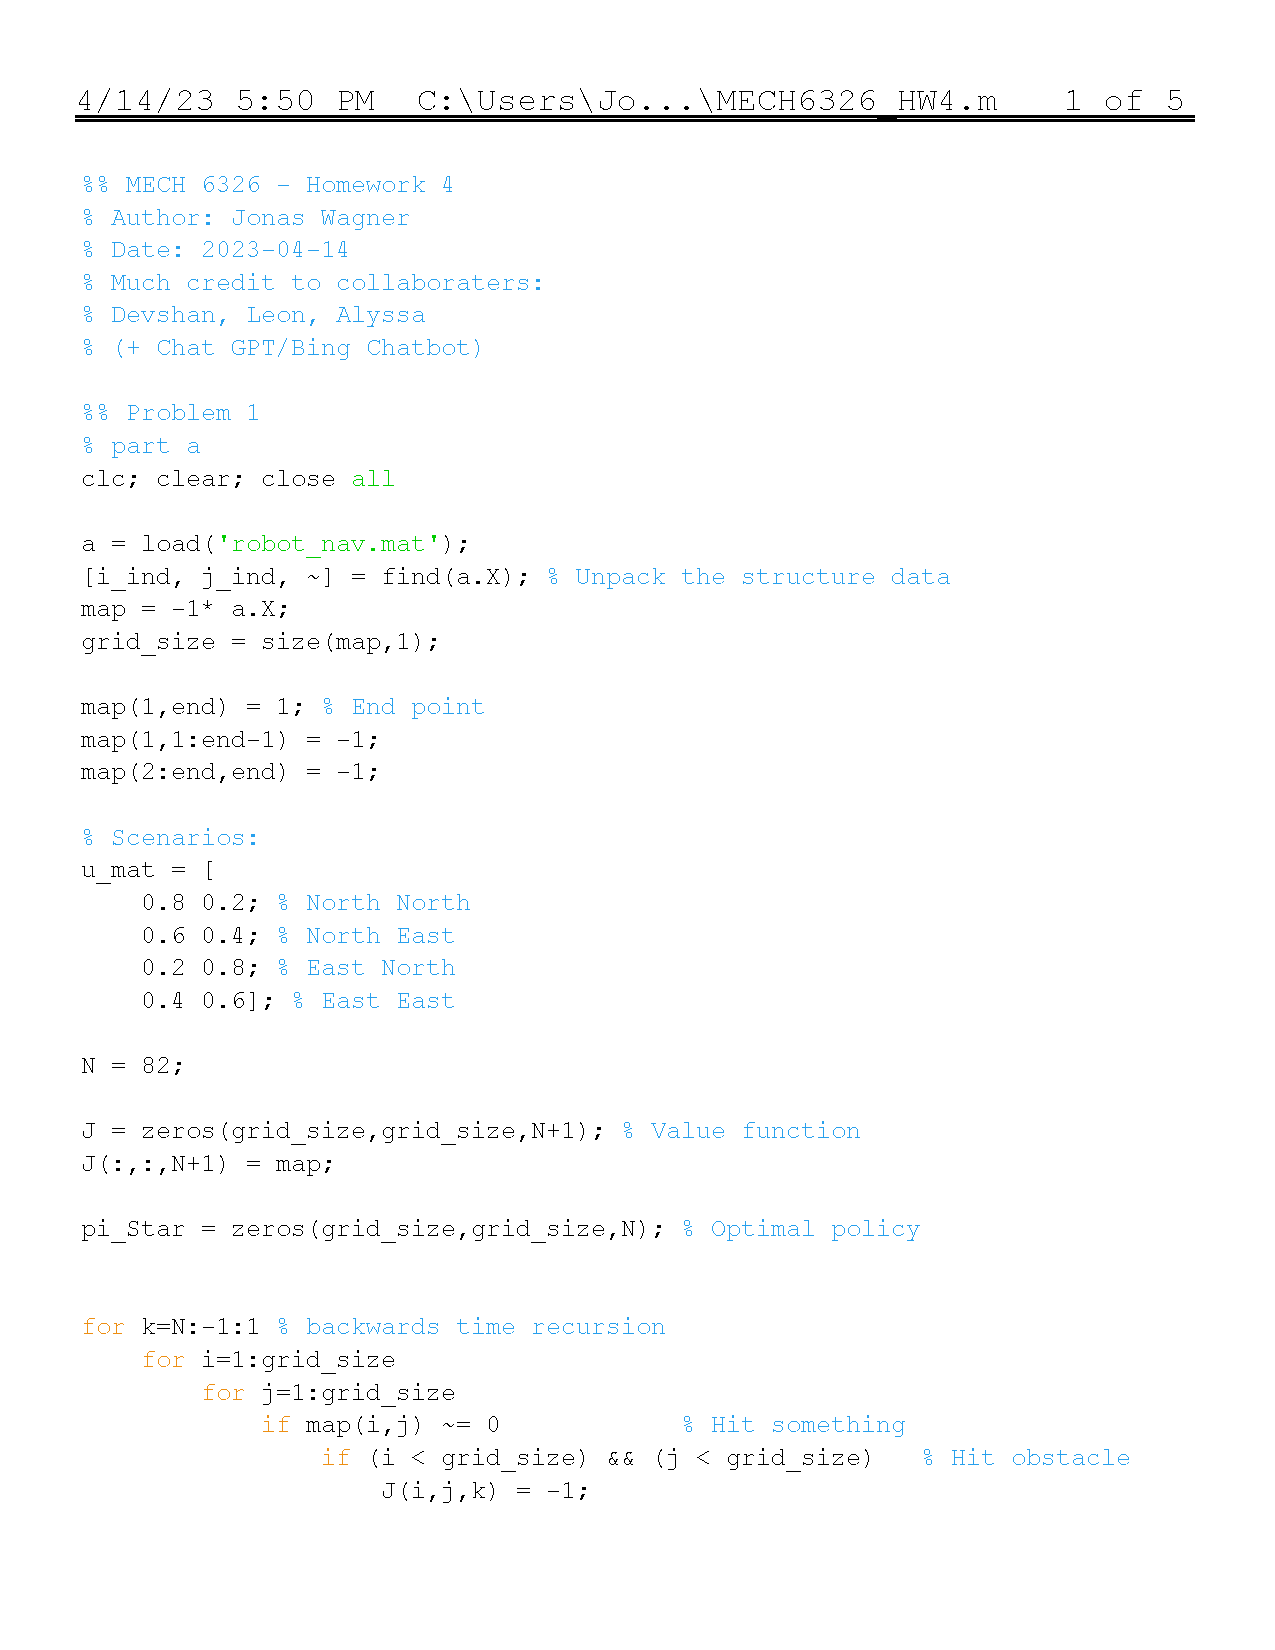
\includepdf[pages=-]{MECH6326_HW4.pdf}
% \newpage
% 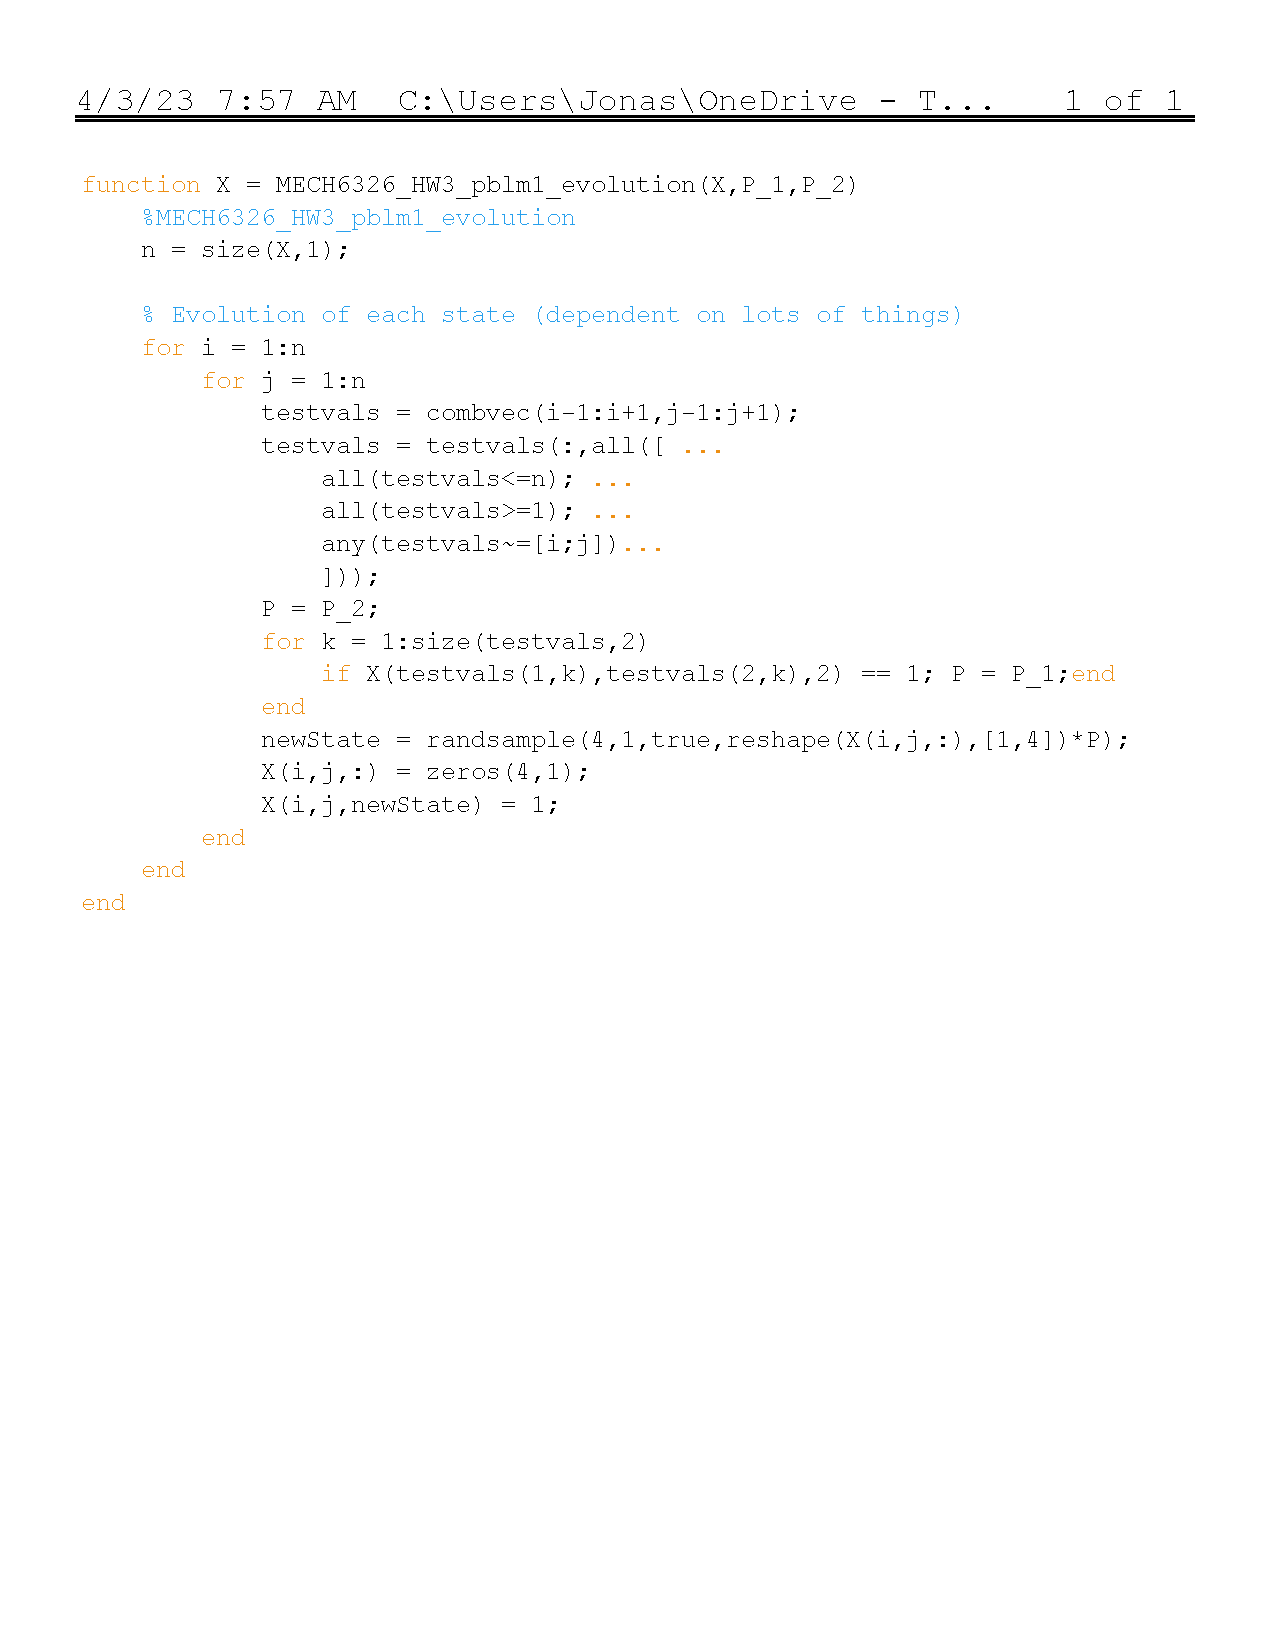
\includepdf[pages=-]{MECH6326_HW3_pblm1_evolution.pdf}

% % Appendix ----------------------------------------------
% \newpage
% \appendix
% \bibliographystyle{plain}
% \bibliography{refs.bib}




\end{document}

